\documentclass[
	letterpaper, % Paper size, specify a4paper (A4) or letterpaper (US letter)
	10pt, % Default font size, specify 10pt, 11pt or 12pt
]{CSUniSchoolLabReport}

\usepackage{fancyvrb}
\usepackage{multicol}
\usepackage{subcaption}

\captionsetup[subfigure]{labelformat=empty}

\title{Analyzing radioactive decay of multiple samples with different half lives.}

\author{Sebastien \textsc{Psarianos}\\ Sofiya \textsc{P'yavka}}

\date{\today}

\begin{document}

\maketitle

\begin{center}
	\begin{tabular}{l r}
		Date Performed: & September 13, 2022 \\
	\end{tabular}
\end{center}

\section{Methods and Procedure}
\textbf{Background Radiation} A Geiger counter was set up in the laboratory with no radioactive sample present. Particle count measurements were taken for every $20$ second interval and this was repeated for $1200$ seconds ($60\times20$ second intervals). The data collected in this portion of the laboratory was used as a baseline measurement for the background radiation in the laboratory.\\

\textbf{Experiment 1} (Barium Sample): A sample of Barium-137 was then placed near the Geiger counter. Particle count measurements were taken again over the same intervals as the background radiation measurements ($60\times20$ second intervals).\\

\textbf{Experiment 2} (Fiesta Plate Sample): A fiesta plate with a coating that contains uranium was then placed near the Geiger counter. The same particle count measurements were again taken for $1200$ seconds, however for this experiment, $3$ second intervals were used ($400\times3$ second intervals).
\section{Results}
Note: All curve fitting regression values were calculated using the \lstinline{curve_fit} function from the \lstinline{scipy.optimize module}. Referenced functions, equations and calculations are detailed in the \textbf{Appendix} section in addition to the raw data and calulated uncertainties.
\newpage
{\Large\textbf{Experiment 1}}
\begin{figure}[H]
	\begin{subfigure}{0.45\textwidth}
		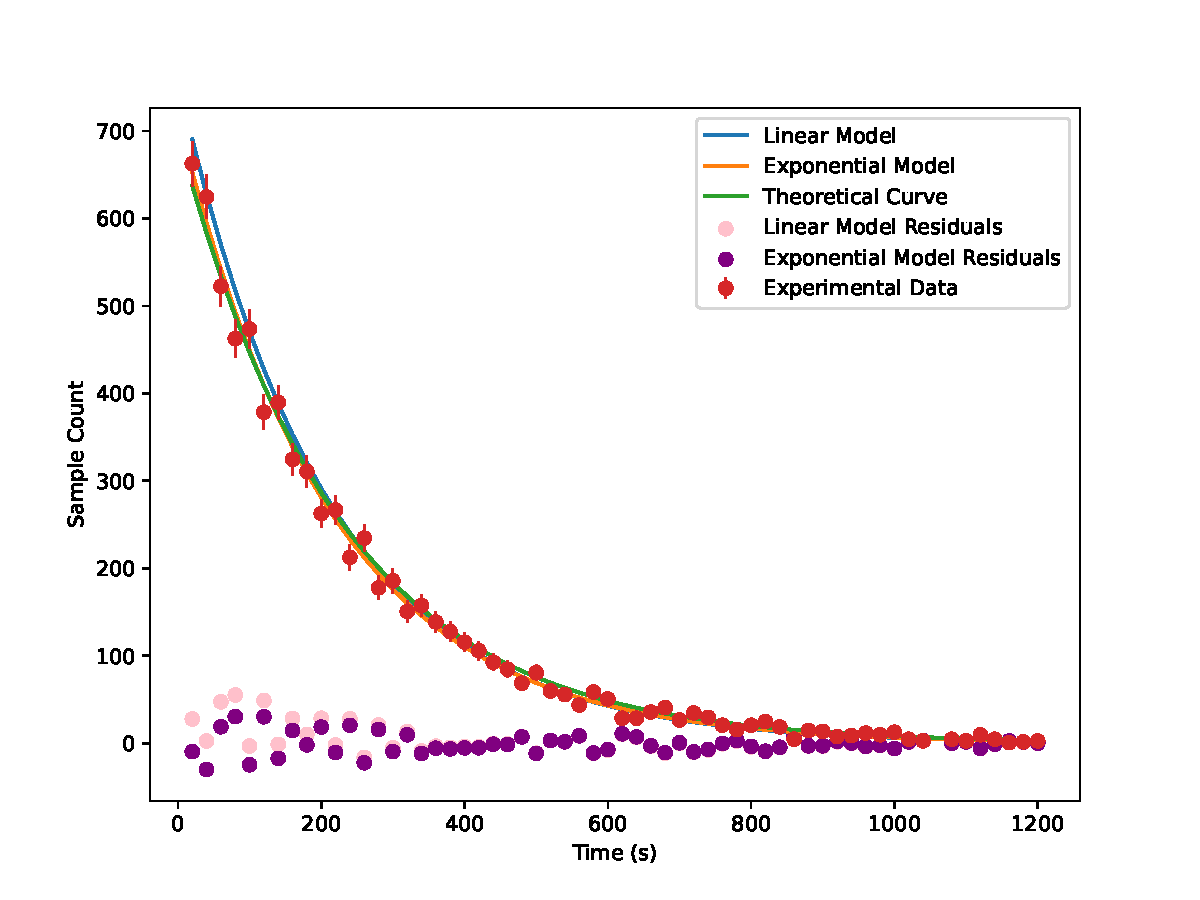
\includegraphics[width=\textwidth]{linearBariumGraph}
		\caption{\textbf{Figure 1: Particle counts over 20 second interval with mean background radiation subtracted vs time for a sample of Barium-137. Linear, exponential and theoretical half life model regressions are included. Residuals for the linear and nonlinear models are included.}}
	\end{subfigure}
	\quad
	\begin{subfigure}{0.45\textwidth}
		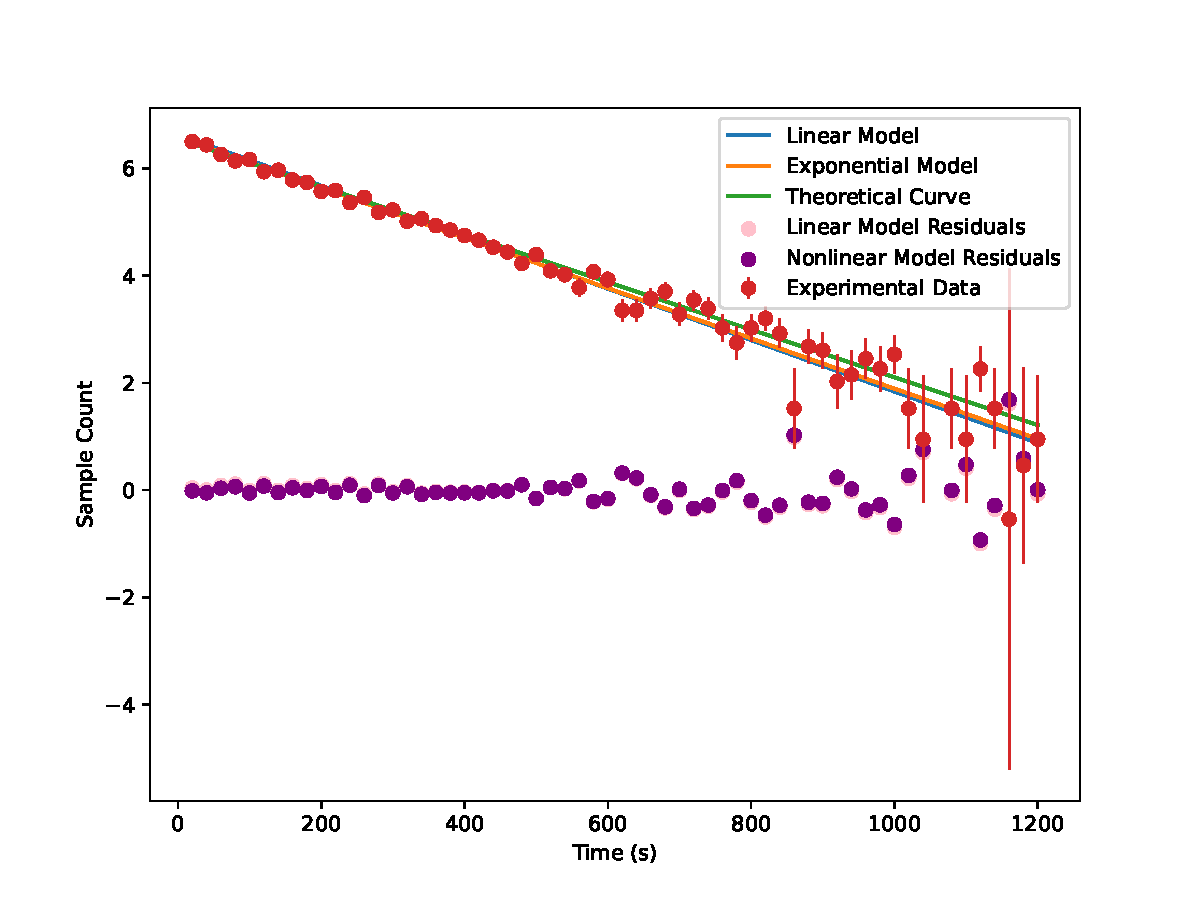
\includegraphics[width=\textwidth]{logBariumGraph}
		\caption{\textbf{Figure 2 Linearized particle counts over 20 second interval with mean background radiation subtracted vs time for a sample of Barium-137.  Linear, exponential and theoretical half life model regressions are included. Residuals for the linear and nonlinear models are included.}}
	\end{subfigure}
\end{figure}
All plotted values have had the mean background radiation measured in the laboratory subtracted from them to approximate actual sample data without background interference. This value is apprximately $3.42$.\\\\
{\large\textbf{Curve fitting}}\\
Three \lstinline{curve_fit} regressions were performed on the data using an exponential model, a linear model and a
model based on the theoretical half life of Barium-137. The derivation of the theoretical model is detailed in
\textbf{Calculation 1}. \textbf{Equation 1}, \textbf{Equation 2} and \textbf{Equation 3} were used for the linear, exponential and
theoretical models respectively. The implementations shown in \textbf{Function 1}, \textbf{Function 2} and \textbf{Function 3} were used for \lstinline{curve_fit}. The exponential
and theoretical model regressions were performed on the raw data set and the linear regression was
performed using the linearized data.\\\\
All data linearization was done using a natural logarithm on the corresponding y-axis. This was used for
linear modelling in addition to the linearized plotting in \textbf{Figure 2} of the data, exponential and theoretical
models. To plot the linear model on \textbf{Figure 1}, the output values of the linear model regression were
converted to nonlinear by taking the exponential of them (base $e$).\\\\
{\large\textbf{Uncertainty Calculations}}\\
Uncertainty in count measurements were all calculated using \textbf{Equation 8}. This was done programmatically
for all measured values using the python implementation \textbf{Function 5}. Sample calculations for the first reading
are shown in \textbf{Calculation 2}.\\\\
Uncertainty was propagated for the linearization by using the logarithmic error propagation shown in
\textbf{Equation 6}. This again was done programmatically for all values using the python implementation \textbf{Function 4}.
Sample calculations for the first reading are shown in \textbf{Calculation 3}\\\\
{\Large\textbf{Experiment 2}}
\begin{figure}[H]
	\begin{subfigure}{0.45\textwidth}
		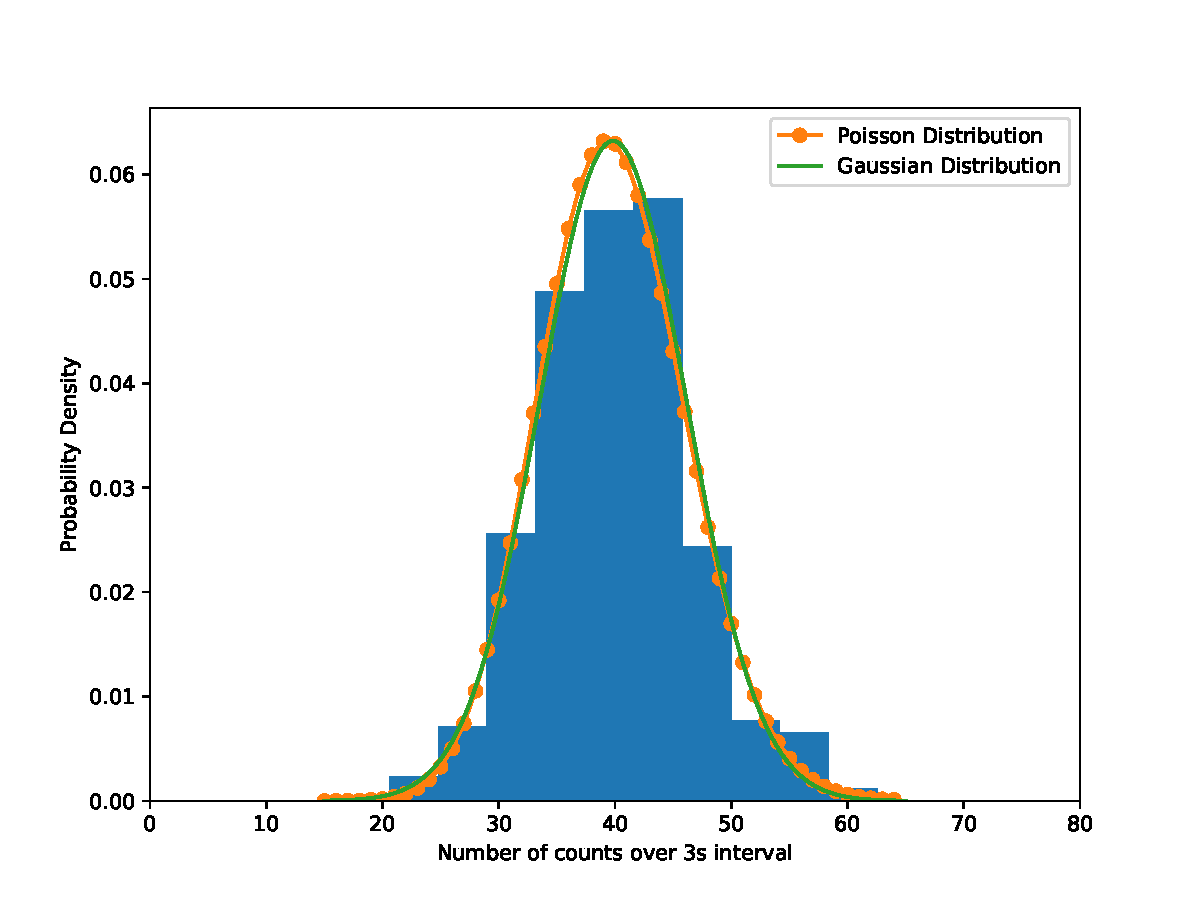
\includegraphics[width=\textwidth]{fiestaDistributionGraph}
		\caption{\textbf{Figure 3: Probability density for various ranges of counts measured over 3s intervals. Data is from the fiesta plate sample measurements. Includes both Poisson and Gaussian distributions. }}
	\end{subfigure}
	\quad
	\begin{subfigure}{0.45\textwidth}
		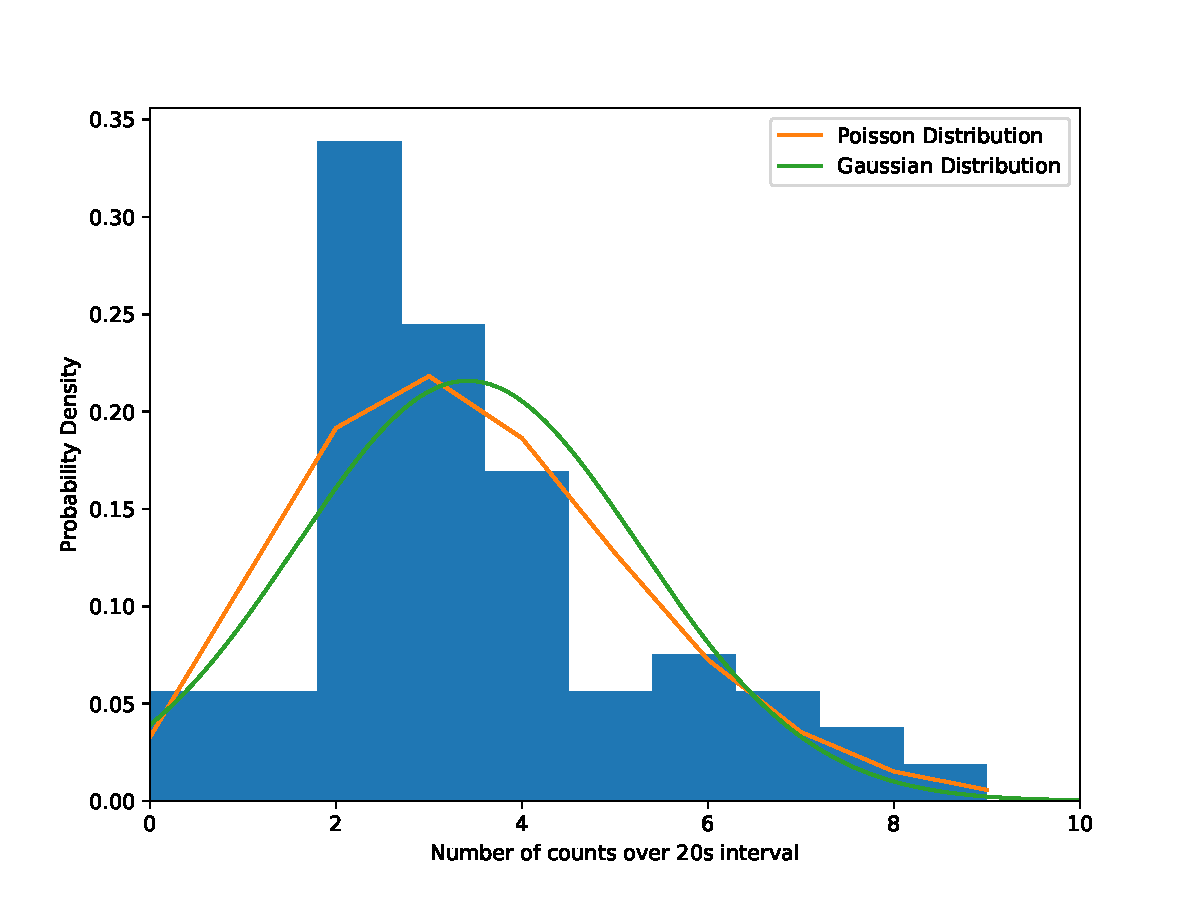
\includegraphics[width=\textwidth]{backgroundDistributionGraph}
		\caption{\textbf{Figure 4: Probability density for various ranges of counts measured over 20s intervals. Data is from the background radiation sample measurements. Includes both Poisson and Gaussian distributions. }}
	\end{subfigure}
\end{figure}
{\large\textbf{Histograms}}\\
Histogram plots in \textbf{Figure 3} and \textbf{Figure 4} were done using the \lstinline{hst} function from the \lstinline{matplotlib.pyplot}
package with the \lstinline{density} set to true, generating a probability density histogram rather than a count
histogram. All binning was done automatically by the \lstinline{hst} function. The plot in \textbf{Figure 3} shows the count
values after the mean background radiation had been subtracted.\\\\
{\large\textbf{Gaussian and Poisson Distributions}}\\
For the Poisson distributions, the \lstinline{poisson.pmf} function from \lstinline{scipy.stats} was used. This function is an implementation of the Poisson probability mass function (\textbf{Equation 9}). For both the background and fiesta plate datasets, the provided $\mu$ value was the mean radiation that was detected over the course of the respective experiment.\\

For the Gaussian distributions, the \lstinline{norm.pdf} function from \lstinline{scipy.stats} was used. This function uses the probability density function (\textbf{Equation 10}) to generate a normal distribution. The scale and location for each distribution was set based on the average count over the respective experiment ($\mu$). One standard deviation ($\sigma$) was set to $\sqrt\mu$ and the location of the distribution was set to $\mu$.
\newpage
\section{Analysis}
\section{Discussion}
\section{Conclusion}
\newpage
\section{Appendix}
{\Large\textbf{Equations}}\\
\begin{tabular}{p{0.45\linewidth} p{0.45\linewidth}}
$$f(x) = ax+b$$
\begin{center}
	\textbf{Equation 1: Linear Model}
\end{center}
&
$$f(x) = ax^b$$
\begin{center}
	\textbf{Equation 2: Exponential Model}
\end{center}\\

$$I(t)= I_0 e^{-\frac{t \ln{2}}{156}}$$
\begin{center}
	\textbf{Equation 3: Theoretical Model}
\end{center}
&
$$I(t) = I_0e^{-\frac{t}{\tau}}$$
\begin{center}
	\textbf{Equation 4: Mean isotope lifetime equation}\\
\end{center}\\

$$\tau = \frac{t_{1/2}}{\ln{2}}$$
\begin{center}
	\textbf{Equation 5: Mean isotope lifetime to half life conversion}
\end{center}
&
$$ u\left(\ln(x_i)\right) = \pm\left|\frac{u(x_i)}{x_i}\right|$$
\begin{center}
	\textbf{Equation 6: Error Propagation for logarithms}
\end{center}\\

$$\chi^2 = \sum_{i=1}^N\left(\frac{y_i-y(x_i)}{u(y_i)}\right)$$
\begin{center}
	\textbf{Equation 7: Chi-Squared Metric}
\end{center}
&
$$u(N_i) = \pm\sqrt{N_{total, i} + \bar{N}_{b}}$$
\begin{center}
	\textbf{Equation 8: Geiger Counter Uncertainty}
\end{center}\\
$$P_\mu(n) = e^{-\mu} \frac{\mu^n}{\Gamma(n+1)}$$
\begin{center}
	\textbf{Equation 9: Poisson mass distribution function}
\end{center}
&
$$f(x) = \frac{e^{-x^2/2}}{\sqrt{2\pi}}$$
\begin{center}
	\textbf{Equation 10: Gaussian probability density function}
\end{center}
\end{tabular}
\vspace{20pt}\\
{\Large\textbf{Python Functions}}
\vspace{20pt}\\
{\large\textbf{Models}}
\begin{verbatim}
def linear_model(values, a, b) -> any:
     return a * values + b
\end{verbatim}
\begin{center}
	\textbf{Function 1: Linear Model (implements Equation 1)}
\end{center}
\vspace{5pt}
\begin{verbatim}
def exponential_model(values, a, b) -> any:
     return b * np.exp(a * values)
\end{verbatim}
\begin{center}
	\textbf{Function 2: Exponential Model (implements Equation 2)}
\end{center}
\vspace{5pt}
\begin{verbatim}
def theoretical_model(values, b) -> any:
     return b * np.exp((-1 / 156 * np.log(2)) * values)
\end{verbatim}
\begin{center}
	\textbf{Function 3: Theoretical Model (implements Equation 3)}
\end{center}
\vspace{10pt}
{\large\textbf{Uncertainty}}
\begin{verbatim}
def logarithmic_error_propagation(value: any, uncertainty: any) -> float:
     """Return the propogated error for the logarithm of a value"""
     return abs(uncertainty / value)
\end{verbatim}
\begin{center}
	\textbf{Function 4: Logarithmic Error Propagation (implements Equation 6)}
\end{center}
\vspace{10pt}
\begin{verbatim}
def calculate_uncertainty(count, mean_background) -> any:
     """Return the uncertainty of the sample.
     """
     return np.sqrt(count + mean_background)
\end{verbatim}
\begin{center}
	\textbf{Function 5: Function used to calculate count uncertainty values (implements Equation 8)}
\end{center}
\vspace{10pt}
{\large\textbf{Data Analysis}}
\begin{verbatim}
def characterize(y: any, func: any, u: any) -> float:
     """Return the reduced chi-squared metric to determine how well a model
     function fits a given set of data using the measured data <y>, the
     prediction with the model <func> and the uncertainty on each measurement's
     dependent data <u>.
     """
     value = 0

     for i in range(np.size(y)):
          value += ((y[i] - func[i]) ** 2) / (u[i] ** 2)
          i += 1

     return value / (np.size(y) - 2)
\end{verbatim}
\begin{center}
	\textbf{Function 6: Function used to calculate chi-squared metric (implements equation 7)}
\end{center}
\vspace{5pt}
\begin{verbatim}
def count_rate(events, sample_time) -> tuple:
     """Return the count rate and its uncertainty.
     """
     return events / sample_time, np.sqrt(events) / sample_time
\end{verbatim}
\begin{center}
	\textbf{Function 7: Function used to calculate count-rate for experimental data}
\end{center}
\newpage % Probably Remove
{\Large\textbf{Sample Calculations}}
\vspace{20pt}\\
The theoretical model was derived by first combining of \textbf{Equation 4} and \textbf{Equation 5}:
$$I(t) = I_0e^{-\frac{t}{\tau}} \iff I(t) = I_0e^{\frac{t}{-\frac{t_{1/2}}{\ln{2}}}} \iff I(t) = I_0e^{-\frac{t\ln{2}}{t_{1/2}}}$$
The theoretical value for the half-life of Barium ($t_{\frac{1}{2}} = 156s$) was included in the equation:
$$I(t) = I_0e^{-\frac{t\ln{2}}{156}}$$
\begin{center}
	\textbf{Calculation 1: Deriving Theoretical Model}
\end{center}
\vspace{10pt}
All Geiger counter uncertainty calculations are based off of \textbf{Equation 8}. The mean of the background radiation count measured in the lab over each 20 second interval was $\bar{N}_b \approx 3.42$, therefore:
$$u(N_i) = \pm\sqrt{N_{total, i} + 3.42}$$
The first count value $N_1$ measured in experiment 1 was $N_1= 666$. Therefore:
$$u(N_1) = \pm\sqrt{666 + 3.42} = \pm\sqrt{669.42} \approx \pm25.87$$
Uncertainty for all values was calculated in this manner programmatically using \textbf{Function 5} which is an implementation of \textbf{Equation 8}.
\begin{center}
	\textbf{Calculation 2: Sample Geiger Counter uncertainty calculation}
\end{center}
\vspace{10pt}
The error values for the linearized plot were calculated using \textbf{Equation 6}. The first measured count value width background subtracted was $N'_{1} = 662.6$ and the uncertainty of the first measurement $u(N'_1) \approx 25.87$ as shown in \textbf{Calculation 2}. Therefore, by \textbf{Equation 6}:
$$u(\ln(N'_1))= \pm\left|\frac{u(N'_1)}{N'_1}\right|= \pm\left|\frac{25.87}{662.6}\right| \approx \pm0.039$$
\begin{center}
	\textbf{Calculation 3: Sample logarithmic error propagation}
\end{center}
\newpage
{\Large\textbf{Raw Data}}\\
\vspace{20pt}\\
\begin{center}
\begin{tabular}{| p{0.14\textwidth} | p{0.14\textwidth}|}\hline
Time Interval (s) & Total Measured Count\\
\hline
0-20 & $3$\\
20-40 & $5$\\
40-60 & $4$\\
60-80 & $2$\\
80-100 & $3$\\
100-120 & $6$\\
120-140 & $4$\\
140-160 & $2$\\
160-180 & $8$\\
180-200 & $4$\\
200-220 & $2$\\
220-240 & $2$\\
240-260 & $3$\\
260-280 & $2$\\
280-300 & $0$\\
300-320 & $8$\\
320-340 & $2$\\
340-360 & $7$\\
360-380 & $5$\\
380-400 & $3$\\
400-420 & $2$\\
420-440 & $2$\\
440-460 & $4$\\
460-480 & $3$\\
480-500 & $2$\\
500-520 & $2$\\
520-540 & $3$\\
540-560 & $3$\\
560-580 & $6$\\
580-600 & $3$\\
\hline
\end{tabular}\quad
\begin{tabular}{| p{0.14\textwidth} | p{0.14\textwidth}|}\hline
Time Interval (s) & Total Measured Count\\
\hline
600-620 & $2$\\
620-640 & $2$\\
640-660 & $0$\\
660-680 & $3$\\
680-700 & $4$\\
700-720 & $6$\\
720-740 & $4$\\
740-760 & $4$\\
760-780 & $3$\\
780-800 & $7$\\
800-820 & $3$\\
820-840 & $5$\\
840-860 & $2$\\
860-880 & $2$\\
880-900 & $3$\\
900-920 & $2$\\
920-940 & $6$\\
940-960 & $4$\\
960-980 & $2$\\
980-1000 & $9$\\
1000-1020 & $0$\\
1020-1040 & $2$\\
1040-1060 & $6$\\
1060-1080 & $3$\\
1080-1100 & $2$\\
1100-1120 & $4$\\
1120-1140 & $1$\\
1140-1160 & $7$\\
1160-1180 & $1$\\
1180-1200 & $1$\\
\hline
\end{tabular}
\end{center}
\begin{center}
	\textbf{Table 1: Raw data from the background radiation measurement, time intervals and measured counts are shown.}
\end{center}
\begin{tabular}{| p{0.14\textwidth} | p{0.14\textwidth} | p{0.14\textwidth} |}\hline
Time Interval (s) & Total Measured Count & Count without background\\
\hline
0-20 & $666$ & $663\pm 30$\\
20-40 & $628$ & $625\pm 30$\\
40-60 & $526$ & $523\pm 20$\\
60-80 & $466$ & $463\pm 20$\\
80-100 & $477$ & $474\pm 20$\\
100-120 & $382$ & $379\pm 20$\\
120-140 & $393$ & $390\pm 20$\\
140-160 & $328$ & $325\pm 20$\\
160-180 & $314$ & $311\pm 20$\\
180-200 & $266$ & $263\pm 20$\\
200-220 & $270$ & $267\pm 20$\\
220-240 & $216$ & $213\pm 10$\\
240-260 & $238$ & $235\pm 20$\\
260-280 & $181$ & $178\pm 10$\\
280-300 & $189$ & $186\pm 10$\\
300-320 & $154$ & $151\pm 10$\\
320-340 & $161$ & $158\pm 10$\\
340-360 & $142$ & $139\pm 10$\\
360-380 & $131$ & $128\pm 10$\\
380-400 & $119$ & $116\pm 10$\\
400-420 & $109$ & $106\pm 10$\\
420-440 & $96$ & $93\pm 10$\\
440-460 & $88$ & $85\pm 10$\\
460-480 & $72$ & $69\pm 9$\\
480-500 & $84$ & $81\pm 9$\\
500-520 & $63$ & $60\pm 8$\\
520-540 & $59$ & $56\pm 8$\\
540-560 & $47$ & $44\pm 7$\\
560-580 & $62$ & $59\pm 8$\\
580-600 & $54$ & $51\pm 8$\\
\hline
\end{tabular}\quad
\begin{tabular}{| p{0.14\textwidth} | p{0.14\textwidth} | p{0.14\textwidth} |}\hline
Time Interval (s) & Total Measured Count & Count without background\\
\hline
600-620 & $32$ & $29\pm 6$\\
620-640 & $32$ & $29\pm 6$\\
640-660 & $39$ & $36\pm 7$\\
660-680 & $44$ & $41\pm 7$\\
680-700 & $30$ & $27\pm 6$\\
700-720 & $38$ & $35\pm 6$\\
720-740 & $33$ & $30\pm 6$\\
740-760 & $24$ & $21\pm 5$\\
760-780 & $19$ & $16\pm 5$\\
780-800 & $24$ & $21\pm 5$\\
800-820 & $28$ & $25\pm 6$\\
820-840 & $22$ & $19\pm 5$\\
840-860 & $8$ & $5\pm 3$\\
860-880 & $18$ & $15\pm 5$\\
880-900 & $17$ & $14\pm 5$\\
900-920 & $11$ & $8\pm 4$\\
920-940 & $12$ & $9\pm 4$\\
940-960 & $15$ & $12\pm 4$\\
960-980 & $13$ & $10\pm 4$\\
980-1000 & $16$ & $13\pm 4$\\
1000-1020 & $8$ & $5\pm 3$\\
1020-1040 & $6$ & $3\pm 3$\\
1040-1060 & $3$ & $0\pm 3$\\
1060-1080 & $8$ & $5\pm 3$\\
1080-1100 & $6$ & $3\pm 3$\\
1100-1120 & $13$ & $10\pm 4$\\
1120-1140 & $8$ & $5\pm 3$\\
1140-1160 & $4$ & $1\pm 3$\\
1160-1180 & $5$ & $2\pm 3$\\
1180-1200 & $6$ & $3\pm 3$\\
\hline
\end{tabular}
\begin{center}
	\textbf{Table 2: Raw data from experiment 1 showing time intervals, total measured counts and rounded counts with background subtracted.}
\end{center}
\begin{tabular}{| p{0.14\textwidth} | p{0.14\textwidth} | p{0.14\textwidth} |}\hline
Time Interval (s) & Total Measured Count & Count without background\\
\hline
0-3 & $39$ & $36\pm 7$\\
3-6 & $39$ & $36\pm 7$\\
6-9 & $42$ & $39\pm 7$\\
9-12 & $33$ & $30\pm 6$\\
12-15 & $49$ & $46\pm 7$\\
15-18 & $32$ & $29\pm 6$\\
18-21 & $31$ & $28\pm 6$\\
21-24 & $54$ & $51\pm 8$\\
24-27 & $60$ & $57\pm 8$\\
27-30 & $40$ & $37\pm 7$\\
30-33 & $42$ & $39\pm 7$\\
33-36 & $45$ & $42\pm 7$\\
36-39 & $61$ & $58\pm 8$\\
39-42 & $45$ & $42\pm 7$\\
42-45 & $42$ & $39\pm 7$\\
45-48 & $49$ & $46\pm 7$\\
48-51 & $44$ & $41\pm 7$\\
51-54 & $41$ & $38\pm 7$\\
54-57 & $53$ & $50\pm 8$\\
57-60 & $46$ & $43\pm 7$\\
60-63 & $39$ & $36\pm 7$\\
63-66 & $35$ & $32\pm 6$\\
66-69 & $43$ & $40\pm 7$\\
69-72 & $41$ & $38\pm 7$\\
72-75 & $49$ & $46\pm 7$\\
75-78 & $50$ & $47\pm 7$\\
78-81 & $59$ & $56\pm 8$\\
81-84 & $47$ & $44\pm 7$\\
84-87 & $41$ & $38\pm 7$\\
87-90 & $37$ & $34\pm 6$\\
90-93 & $38$ & $35\pm 6$\\
93-96 & $53$ & $50\pm 8$\\
96-99 & $38$ & $35\pm 6$\\
99-102 & $37$ & $34\pm 6$\\
102-105 & $52$ & $49\pm 7$\\
105-108 & $46$ & $43\pm 7$\\
108-111 & $41$ & $38\pm 7$\\
111-114 & $32$ & $29\pm 6$\\
114-117 & $35$ & $32\pm 6$\\
117-120 & $39$ & $36\pm 7$\\
\hline
\end{tabular}\quad
\begin{tabular}{| p{0.14\textwidth} | p{0.14\textwidth} | p{0.14\textwidth} |}\hline
Time Interval (s) & Total Measured Count & Count without background\\
\hline
120-123 & $39$ & $36\pm 7$\\
123-126 & $39$ & $36\pm 7$\\
126-129 & $34$ & $31\pm 6$\\
129-132 & $46$ & $43\pm 7$\\
132-135 & $42$ & $39\pm 7$\\
135-138 & $39$ & $36\pm 7$\\
138-141 & $52$ & $49\pm 7$\\
141-144 & $51$ & $48\pm 7$\\
144-147 & $59$ & $56\pm 8$\\
147-150 & $42$ & $39\pm 7$\\
150-153 & $52$ & $49\pm 7$\\
153-156 & $36$ & $33\pm 6$\\
156-159 & $48$ & $45\pm 7$\\
159-162 & $47$ & $44\pm 7$\\
162-165 & $44$ & $41\pm 7$\\
165-168 & $41$ & $38\pm 7$\\
168-171 & $37$ & $34\pm 6$\\
171-174 & $53$ & $50\pm 8$\\
174-177 & $45$ & $42\pm 7$\\
177-180 & $52$ & $49\pm 7$\\
180-183 & $44$ & $41\pm 7$\\
183-186 & $42$ & $39\pm 7$\\
186-189 & $53$ & $50\pm 8$\\
189-192 & $47$ & $44\pm 7$\\
192-195 & $51$ & $48\pm 7$\\
195-198 & $45$ & $42\pm 7$\\
198-201 & $41$ & $38\pm 7$\\
201-204 & $46$ & $43\pm 7$\\
204-207 & $39$ & $36\pm 7$\\
207-210 & $54$ & $51\pm 8$\\
210-213 & $51$ & $48\pm 7$\\
213-216 & $45$ & $42\pm 7$\\
216-219 & $35$ & $32\pm 6$\\
219-222 & $44$ & $41\pm 7$\\
222-225 & $46$ & $43\pm 7$\\
225-228 & $40$ & $37\pm 7$\\
228-231 & $44$ & $41\pm 7$\\
231-234 & $47$ & $44\pm 7$\\
234-237 & $37$ & $34\pm 6$\\
237-240 & $36$ & $33\pm 6$\\
\hline
\end{tabular}\\
\begin{tabular}{| p{0.14\textwidth} | p{0.14\textwidth} | p{0.14\textwidth} |}\hline
Time Interval (s) & Total Measured Count & Count without background\\
\hline
240-243 & $40$ & $37\pm 7$\\
243-246 & $32$ & $29\pm 6$\\
246-249 & $51$ & $48\pm 7$\\
249-252 & $40$ & $37\pm 7$\\
252-255 & $33$ & $30\pm 6$\\
255-258 & $45$ & $42\pm 7$\\
258-261 & $37$ & $34\pm 6$\\
261-264 & $58$ & $55\pm 8$\\
264-267 & $50$ & $47\pm 7$\\
267-270 & $37$ & $34\pm 6$\\
270-273 & $38$ & $35\pm 6$\\
273-276 & $48$ & $45\pm 7$\\
276-279 & $49$ & $46\pm 7$\\
279-282 & $39$ & $36\pm 7$\\
282-285 & $40$ & $37\pm 7$\\
285-288 & $45$ & $42\pm 7$\\
288-291 & $43$ & $40\pm 7$\\
291-294 & $55$ & $52\pm 8$\\
294-297 & $37$ & $34\pm 6$\\
297-300 & $36$ & $33\pm 6$\\
300-303 & $40$ & $37\pm 7$\\
303-306 & $40$ & $37\pm 7$\\
306-309 & $38$ & $35\pm 6$\\
309-312 & $43$ & $40\pm 7$\\
312-315 & $51$ & $48\pm 7$\\
315-318 & $49$ & $46\pm 7$\\
318-321 & $58$ & $55\pm 8$\\
321-324 & $36$ & $33\pm 6$\\
324-327 & $47$ & $44\pm 7$\\
327-330 & $41$ & $38\pm 7$\\
330-333 & $43$ & $40\pm 7$\\
333-336 & $48$ & $45\pm 7$\\
336-339 & $42$ & $39\pm 7$\\
339-342 & $50$ & $47\pm 7$\\
342-345 & $53$ & $50\pm 8$\\
345-348 & $49$ & $46\pm 7$\\
348-351 & $51$ & $48\pm 7$\\
351-354 & $41$ & $38\pm 7$\\
354-357 & $45$ & $42\pm 7$\\
357-360 & $37$ & $34\pm 6$\\
\hline
\end{tabular}\quad
\begin{tabular}{| p{0.14\textwidth} | p{0.14\textwidth} | p{0.14\textwidth} |}\hline
Time Interval (s) & Total Measured Count & Count without background\\
\hline
360-363 & $30$ & $27\pm 6$\\
363-366 & $40$ & $37\pm 7$\\
366-369 & $44$ & $41\pm 7$\\
369-372 & $47$ & $44\pm 7$\\
372-375 & $48$ & $45\pm 7$\\
375-378 & $41$ & $38\pm 7$\\
378-381 & $34$ & $31\pm 6$\\
381-384 & $41$ & $38\pm 7$\\
384-387 & $41$ & $38\pm 7$\\
387-390 & $43$ & $40\pm 7$\\
390-393 & $47$ & $44\pm 7$\\
393-396 & $45$ & $42\pm 7$\\
396-399 & $39$ & $36\pm 7$\\
399-402 & $47$ & $44\pm 7$\\
402-405 & $45$ & $42\pm 7$\\
405-408 & $27$ & $24\pm 6$\\
408-411 & $50$ & $47\pm 7$\\
411-414 & $47$ & $44\pm 7$\\
414-417 & $44$ & $41\pm 7$\\
417-420 & $47$ & $44\pm 7$\\
420-423 & $46$ & $43\pm 7$\\
423-426 & $48$ & $45\pm 7$\\
426-429 & $33$ & $30\pm 6$\\
429-432 & $34$ & $31\pm 6$\\
432-435 & $42$ & $39\pm 7$\\
435-438 & $43$ & $40\pm 7$\\
438-441 & $39$ & $36\pm 7$\\
441-444 & $46$ & $43\pm 7$\\
444-447 & $38$ & $35\pm 6$\\
447-450 & $40$ & $37\pm 7$\\
450-453 & $36$ & $33\pm 6$\\
453-456 & $49$ & $46\pm 7$\\
456-459 & $50$ & $47\pm 7$\\
459-462 & $40$ & $37\pm 7$\\
462-465 & $50$ & $47\pm 7$\\
465-468 & $53$ & $50\pm 8$\\
468-471 & $54$ & $51\pm 8$\\
471-474 & $37$ & $34\pm 6$\\
474-477 & $41$ & $38\pm 7$\\
477-480 & $44$ & $41\pm 7$\\
\hline
\end{tabular}\\
\begin{tabular}{| p{0.14\textwidth} | p{0.14\textwidth} | p{0.14\textwidth} |}\hline
Time Interval (s) & Total Measured Count & Count without background\\
\hline
480-483 & $58$ & $55\pm 8$\\
483-486 & $42$ & $39\pm 7$\\
486-489 & $51$ & $48\pm 7$\\
489-492 & $41$ & $38\pm 7$\\
492-495 & $50$ & $47\pm 7$\\
495-498 & $45$ & $42\pm 7$\\
498-501 & $41$ & $38\pm 7$\\
501-504 & $42$ & $39\pm 7$\\
504-507 & $48$ & $45\pm 7$\\
507-510 & $42$ & $39\pm 7$\\
510-513 & $39$ & $36\pm 7$\\
513-516 & $50$ & $47\pm 7$\\
516-519 & $47$ & $44\pm 7$\\
519-522 & $49$ & $46\pm 7$\\
522-525 & $47$ & $44\pm 7$\\
525-528 & $33$ & $30\pm 6$\\
528-531 & $37$ & $34\pm 6$\\
531-534 & $52$ & $49\pm 7$\\
534-537 & $46$ & $43\pm 7$\\
537-540 & $38$ & $35\pm 6$\\
540-543 & $42$ & $39\pm 7$\\
543-546 & $37$ & $34\pm 6$\\
546-549 & $30$ & $27\pm 6$\\
549-552 & $48$ & $45\pm 7$\\
552-555 & $47$ & $44\pm 7$\\
555-558 & $38$ & $35\pm 6$\\
558-561 & $41$ & $38\pm 7$\\
561-564 & $34$ & $31\pm 6$\\
564-567 & $35$ & $32\pm 6$\\
567-570 & $36$ & $33\pm 6$\\
570-573 & $39$ & $36\pm 7$\\
573-576 & $36$ & $33\pm 6$\\
576-579 & $43$ & $40\pm 7$\\
579-582 & $55$ & $52\pm 8$\\
582-585 & $43$ & $40\pm 7$\\
585-588 & $45$ & $42\pm 7$\\
588-591 & $32$ & $29\pm 6$\\
591-594 & $51$ & $48\pm 7$\\
594-597 & $45$ & $42\pm 7$\\
597-600 & $57$ & $54\pm 8$\\
\hline
\end{tabular}\quad
\begin{tabular}{| p{0.14\textwidth} | p{0.14\textwidth} | p{0.14\textwidth} |}\hline
Time Interval (s) & Total Measured Count & Count without background\\
\hline
600-603 & $32$ & $29\pm 6$\\
603-606 & $48$ & $45\pm 7$\\
606-609 & $47$ & $44\pm 7$\\
609-612 & $42$ & $39\pm 7$\\
612-615 & $24$ & $21\pm 5$\\
615-618 & $55$ & $52\pm 8$\\
618-621 & $54$ & $51\pm 8$\\
621-624 & $43$ & $40\pm 7$\\
624-627 & $48$ & $45\pm 7$\\
627-630 & $43$ & $40\pm 7$\\
630-633 & $59$ & $56\pm 8$\\
633-636 & $33$ & $30\pm 6$\\
636-639 & $41$ & $38\pm 7$\\
639-642 & $45$ & $42\pm 7$\\
642-645 & $54$ & $51\pm 8$\\
645-648 & $36$ & $33\pm 6$\\
648-651 & $40$ & $37\pm 7$\\
651-654 & $41$ & $38\pm 7$\\
654-657 & $54$ & $51\pm 8$\\
657-660 & $42$ & $39\pm 7$\\
660-663 & $42$ & $39\pm 7$\\
663-666 & $46$ & $43\pm 7$\\
666-669 & $43$ & $40\pm 7$\\
669-672 & $30$ & $27\pm 6$\\
672-675 & $46$ & $43\pm 7$\\
675-678 & $47$ & $44\pm 7$\\
678-681 & $39$ & $36\pm 7$\\
681-684 & $55$ & $52\pm 8$\\
684-687 & $45$ & $42\pm 7$\\
687-690 & $47$ & $44\pm 7$\\
690-693 & $46$ & $43\pm 7$\\
693-696 & $50$ & $47\pm 7$\\
696-699 & $40$ & $37\pm 7$\\
699-702 & $44$ & $41\pm 7$\\
702-705 & $66$ & $63\pm 8$\\
705-708 & $39$ & $36\pm 7$\\
708-711 & $43$ & $40\pm 7$\\
711-714 & $42$ & $39\pm 7$\\
714-717 & $55$ & $52\pm 8$\\
717-720 & $41$ & $38\pm 7$\\
\hline
\end{tabular}\\
\begin{tabular}{| p{0.14\textwidth} | p{0.14\textwidth} | p{0.14\textwidth} |}\hline
Time Interval (s) & Total Measured Count & Count without background\\
\hline
720-723 & $49$ & $46\pm 7$\\
723-726 & $58$ & $55\pm 8$\\
726-729 & $45$ & $42\pm 7$\\
729-732 & $47$ & $44\pm 7$\\
732-735 & $42$ & $39\pm 7$\\
735-738 & $61$ & $58\pm 8$\\
738-741 & $44$ & $41\pm 7$\\
741-744 & $35$ & $32\pm 6$\\
744-747 & $39$ & $36\pm 7$\\
747-750 & $44$ & $41\pm 7$\\
750-753 & $35$ & $32\pm 6$\\
753-756 & $41$ & $38\pm 7$\\
756-759 & $53$ & $50\pm 8$\\
759-762 & $47$ & $44\pm 7$\\
762-765 & $63$ & $60\pm 8$\\
765-768 & $35$ & $32\pm 6$\\
768-771 & $47$ & $44\pm 7$\\
771-774 & $36$ & $33\pm 6$\\
774-777 & $37$ & $34\pm 6$\\
777-780 & $33$ & $30\pm 6$\\
780-783 & $43$ & $40\pm 7$\\
783-786 & $33$ & $30\pm 6$\\
786-789 & $44$ & $41\pm 7$\\
789-792 & $44$ & $41\pm 7$\\
792-795 & $39$ & $36\pm 7$\\
795-798 & $41$ & $38\pm 7$\\
798-801 & $48$ & $45\pm 7$\\
801-804 & $34$ & $31\pm 6$\\
804-807 & $36$ & $33\pm 6$\\
807-810 & $40$ & $37\pm 7$\\
810-813 & $41$ & $38\pm 7$\\
813-816 & $38$ & $35\pm 6$\\
816-819 & $43$ & $40\pm 7$\\
819-822 & $46$ & $43\pm 7$\\
822-825 & $39$ & $36\pm 7$\\
825-828 & $37$ & $34\pm 6$\\
828-831 & $44$ & $41\pm 7$\\
831-834 & $47$ & $44\pm 7$\\
834-837 & $46$ & $43\pm 7$\\
837-840 & $42$ & $39\pm 7$\\
\hline
\end{tabular}\quad
\begin{tabular}{| p{0.14\textwidth} | p{0.14\textwidth} | p{0.14\textwidth} |}\hline
Time Interval (s) & Total Measured Count & Count without background\\
\hline
840-843 & $36$ & $33\pm 6$\\
843-846 & $34$ & $31\pm 6$\\
846-849 & $50$ & $47\pm 7$\\
849-852 & $53$ & $50\pm 8$\\
852-855 & $24$ & $21\pm 5$\\
855-858 & $48$ & $45\pm 7$\\
858-861 & $49$ & $46\pm 7$\\
861-864 & $45$ & $42\pm 7$\\
864-867 & $50$ & $47\pm 7$\\
867-870 & $27$ & $24\pm 6$\\
870-873 & $33$ & $30\pm 6$\\
873-876 & $47$ & $44\pm 7$\\
876-879 & $37$ & $34\pm 6$\\
879-882 & $41$ & $38\pm 7$\\
882-885 & $45$ & $42\pm 7$\\
885-888 & $41$ & $38\pm 7$\\
888-891 & $49$ & $46\pm 7$\\
891-894 & $31$ & $28\pm 6$\\
894-897 & $41$ & $38\pm 7$\\
897-900 & $51$ & $48\pm 7$\\
900-903 & $36$ & $33\pm 6$\\
903-906 & $43$ & $40\pm 7$\\
906-909 & $48$ & $45\pm 7$\\
909-912 & $43$ & $40\pm 7$\\
912-915 & $46$ & $43\pm 7$\\
915-918 & $40$ & $37\pm 7$\\
918-921 & $48$ & $45\pm 7$\\
921-924 & $37$ & $34\pm 6$\\
924-927 & $40$ & $37\pm 7$\\
927-930 & $46$ & $43\pm 7$\\
930-933 & $44$ & $41\pm 7$\\
933-936 & $39$ & $36\pm 7$\\
936-939 & $45$ & $42\pm 7$\\
939-942 & $39$ & $36\pm 7$\\
942-945 & $40$ & $37\pm 7$\\
945-948 & $40$ & $37\pm 7$\\
948-951 & $39$ & $36\pm 7$\\
951-954 & $44$ & $41\pm 7$\\
954-957 & $45$ & $42\pm 7$\\
957-960 & $37$ & $34\pm 6$\\
\hline
\end{tabular}\\
\begin{tabular}{| p{0.14\textwidth} | p{0.14\textwidth} | p{0.14\textwidth} |}\hline
Time Interval (s) & Total Measured Count & Count without background\\
\hline
960-963 & $44$ & $41\pm 7$\\
963-966 & $40$ & $37\pm 7$\\
966-969 & $41$ & $38\pm 7$\\
969-972 & $54$ & $51\pm 8$\\
972-975 & $37$ & $34\pm 6$\\
975-978 & $35$ & $32\pm 6$\\
978-981 & $50$ & $47\pm 7$\\
981-984 & $39$ & $36\pm 7$\\
984-987 & $38$ & $35\pm 6$\\
987-990 & $38$ & $35\pm 6$\\
990-993 & $53$ & $50\pm 8$\\
993-996 & $43$ & $40\pm 7$\\
996-999 & $49$ & $46\pm 7$\\
999-1002 & $33$ & $30\pm 6$\\
1002-1005 & $39$ & $36\pm 7$\\
1005-1008 & $40$ & $37\pm 7$\\
1008-1011 & $49$ & $46\pm 7$\\
1011-1014 & $45$ & $42\pm 7$\\
1014-1017 & $40$ & $37\pm 7$\\
1017-1020 & $35$ & $32\pm 6$\\
1020-1023 & $46$ & $43\pm 7$\\
1023-1026 & $44$ & $41\pm 7$\\
1026-1029 & $40$ & $37\pm 7$\\
1029-1032 & $50$ & $47\pm 7$\\
1032-1035 & $42$ & $39\pm 7$\\
1035-1038 & $35$ & $32\pm 6$\\
1038-1041 & $32$ & $29\pm 6$\\
1041-1044 & $51$ & $48\pm 7$\\
1044-1047 & $58$ & $55\pm 8$\\
1047-1050 & $46$ & $43\pm 7$\\
1050-1053 & $47$ & $44\pm 7$\\
1053-1056 & $47$ & $44\pm 7$\\
1056-1059 & $42$ & $39\pm 7$\\
1059-1062 & $44$ & $41\pm 7$\\
1062-1065 & $43$ & $40\pm 7$\\
1065-1068 & $39$ & $36\pm 7$\\
1068-1071 & $42$ & $39\pm 7$\\
1071-1074 & $45$ & $42\pm 7$\\
1074-1077 & $36$ & $33\pm 6$\\
1077-1080 & $40$ & $37\pm 7$\\
\hline
\end{tabular}\quad
\begin{tabular}{| p{0.14\textwidth} | p{0.14\textwidth} | p{0.14\textwidth} |}\hline
Time Interval (s) & Total Measured Count & Count without background\\
\hline
1080-1083 & $38$ & $35\pm 6$\\
1083-1086 & $42$ & $39\pm 7$\\
1086-1089 & $35$ & $32\pm 6$\\
1089-1092 & $38$ & $35\pm 6$\\
1092-1095 & $39$ & $36\pm 7$\\
1095-1098 & $49$ & $46\pm 7$\\
1098-1101 & $51$ & $48\pm 7$\\
1101-1104 & $44$ & $41\pm 7$\\
1104-1107 & $38$ & $35\pm 6$\\
1107-1110 & $39$ & $36\pm 7$\\
1110-1113 & $44$ & $41\pm 7$\\
1113-1116 & $43$ & $40\pm 7$\\
1116-1119 & $31$ & $28\pm 6$\\
1119-1122 & $52$ & $49\pm 7$\\
1122-1125 & $48$ & $45\pm 7$\\
1125-1128 & $43$ & $40\pm 7$\\
1128-1131 & $35$ & $32\pm 6$\\
1131-1134 & $51$ & $48\pm 7$\\
1134-1137 & $44$ & $41\pm 7$\\
1137-1140 & $44$ & $41\pm 7$\\
1140-1143 & $46$ & $43\pm 7$\\
1143-1146 & $38$ & $35\pm 6$\\
1146-1149 & $48$ & $45\pm 7$\\
1149-1152 & $46$ & $43\pm 7$\\
1152-1155 & $42$ & $39\pm 7$\\
1155-1158 & $52$ & $49\pm 7$\\
1158-1161 & $40$ & $37\pm 7$\\
1161-1164 & $46$ & $43\pm 7$\\
1164-1167 & $41$ & $38\pm 7$\\
1167-1170 & $44$ & $41\pm 7$\\
1170-1173 & $40$ & $37\pm 7$\\
1173-1176 & $45$ & $42\pm 7$\\
1176-1179 & $44$ & $41\pm 7$\\
1179-1182 & $33$ & $30\pm 6$\\
1182-1185 & $40$ & $37\pm 7$\\
1185-1188 & $42$ & $39\pm 7$\\
1188-1191 & $45$ & $42\pm 7$\\
1191-1194 & $33$ & $30\pm 6$\\
1194-1197 & $34$ & $31\pm 6$\\
1197-1200 & $48$ & $45\pm 7$\\
\hline
\end{tabular}
\begin{center}
	\textbf{Table 3: Raw data from experiment 2 showing time intervals, total measured counts and rounded counts with background subtracted.}
\end{center}
\end{document}